\section{Spannungsversorgung}\label{sec.spannungsversorgung}
In diesem Abschnitt soll auf die hardwareseitige Umsetzung der Spannungsversorgung für die Wetterstation eingegangen werden. Ziel ist der Entwurf einer Platine, auf der sämtliche Anforderungen umgesetzt werden.

\subsection{Anforderungen}\label{subsec.anforderungen}
Zunächst sollen in diesem Abschnitt die Anforderungen, die sich aus der Aufgabenstellung ableiten lassen, sowie solche, die sich aus den weiteren Überlegungen zur Umsetzung der Wetterstation ergeben.

\begin{itemize}

	\item Messung des Ladestroms
	\item Messung der Batteriespannung (Ladezustand)
	\item Messung des Stromverbrauchs der Wetterstation

\end{itemize}

Des Weiteren soll der Stromverbrauch der Wetterstation so niedrig wie möglich sein, um die Puffer-Batterie zu schonen und sonnenarme Phasen bzw. die Nacht ohne Stromausfall überbrücken zu können. Die verwendete Batterie hat eine Ladeschlussspannung von 12\,V. Da für den Mikrocontroller und die Sensoren allerdings Spannungspegel von 3,3\,V und 5\,V benötigt werden, müssen diese auf der Platine erzeugt werden.

Aus den mechanischen Anforderungen, dass Mikrocontroller, Platine und Sensoren möglichst in einem Gehäuse untergebracht werden sollen, ergibt sich, dass die entworfene Platine auf die Pinheader des Mikrocontrollers gesteckt werden soll.

\subsection{Erzeugung benötigter Spannungen}\label{subsec.Spannungserzeugung}
Wie in \ref{subsec.anforderungen} beschrieben, werden sowohl 3,3V als auch 5V-Pegel für die Wetterstation benötigt. Angestrebt ist, dass die verwendeten Buck-Spannungsregler eine möglichst geringe Ruhestromaufnahme und einen guten Wirkungsgrad haben. Die Wahr fiel hierbei auf den \textit{LTC3621}. Dieser hat einen Eingangsspannungsbereich von 2,7\,V bis 17\,V und eine Ausgangsspannung, die sich über einen Spannungsteiler am Feedback-Pin zwischen 0,6\,V und der Eingangsspannung einstellen lässt. Der Ruhestrom beträgt laut Datenblatt 3,5\,$\mu$A ~\cite{ltc3621}. Der Regler kann einen maximalen Ausgangsstrom von 1\,A liefern. Da bei der Wahl des Spannungsreglers noch keine Werte über die von der Peripherie benötigte Leistung vorlag, ist dieser Wert eventuell etwas überdimensioniert.

Die Beschaltung des Reglers entspricht den Empfehlungen des Datenblatts, wie sie in Abbildung \ref{fig.ltc3621} dargestellt ist:

\begin{figure}[H]
  \centering
  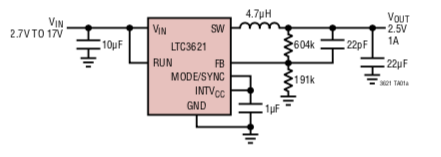
\includegraphics[width=0.6\textwidth]{./img/ltc3621.png}
  \caption{Darstellung des LTC3621 mit beispielhafter Beschaltung gemäß Datenblatt~\cite{ltc3621}}\label{fig.ltc3621}
\end{figure}

Zusätzlich verfügt dieser Regler über die Option, über einen Befehl des Mikrocontrollers manuell ein- bzw. ausgeschaltet zu werden, was weiterhin günstig für den Gesamtstromverbrauch ist.

\subsubsection{3V3}\label{subsubsec.3v3}
Im folgenden soll hauptsächlich auf die Dimensionierung des Spannungsteilers zur Erzeugung von 3,3\,V eingegangen werden. Der Regler hat dabei eine interne Referenzspannung am FB-Pin, die 0,6\,V beträgt, über die die Ausgangsspannung geregelt wird. 

\begin{figure}[H]
  \centering
  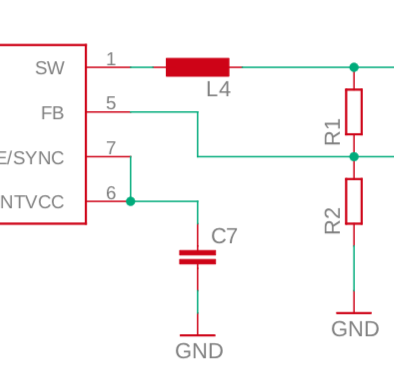
\includegraphics[width=0.4\textwidth]{./img/spannungsteiler_3v3.png}
  \caption{Spannungsteiler am FB-Pins des 3V3 Reglers}\label{fig.spgsteiler3v3}
\end{figure}

Es kann somit der folgende Spannungsteiler aufgestellt werden:

\begin{minipage}{\textwidth}
\begin{equation}\label{eq:Spannungsteiler3v3}
\frac {U_{FB}}{U_a}{=}  \frac{R_{101}}{R_{101}+R_{100}}
\end{equation}
\end{minipage}

Mit $U_{FB}=0,6\,\si{\volt}$, $U_a=3,3\,\si{\volt}$ und $R_{101}=150\,\si{\kilo\ohm}$ ergibt sich:

\begin{minipage}{\textwidth}
\begin{equation}\label{eq:Spannungsteiler3v3b}
\frac {0,6\,\si{\volt}}{3,3\,\si{\volt}}{=}  \frac{150\,\si{\kilo\ohm}}{150\,\si{\kilo\ohm}+R_{100}} \Rightarrow R_{100}=680\,\si{\kilo\ohm}
\end{equation}
\end{minipage}

Der Spannungsteiler wurde hochohmig dimensioniert, um den Stromfluss möglichst klein zu halten.


%Spannungsteiler Formel, was wird alles von 3V3 versorgt 
\subsubsection{5V}\label{subsubsec.5v}
Die Bestimmung des Spannungsteilers für die Erzeugung von 5V erfolgt analog zu Abschnitt \ref{subsubsec.3v3}. Es lässt sich folgender Spannungsteiler aufstellen:

\begin{figure}[H]
  \centering
  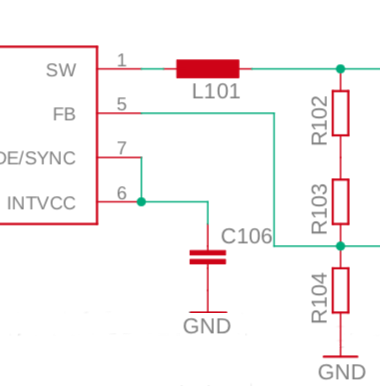
\includegraphics[width=0.4\textwidth]{./img/spannungsteiler_5v.png}
  \caption{Spannungsteiler am FB-Pins des 5V Reglers}\label{fig.spgsteiler5v}
\end{figure}

Dieser wird beschrieben durch:

\begin{minipage}{\textwidth}
\begin{equation}\label{eq:Spannungsteiler5v}
\frac {U_{FB}}{U_a}{=}  \frac{R_{104}}{R_{104}+R_{103}+R_{102}}
\end{equation}
\end{minipage}

Mit $U_{FB}=0,6\,\si{\volt}$, $U_a=3,3\,\si{\volt}$ und $R_{104}=100\,\si{\kilo\ohm}$ ergibt sich:

\begin{minipage}{\textwidth}
\begin{equation}\label{eq:Spannungsteiler5vb}
\frac {0,6\,\si{\volt}}{3,3\,\si{\volt}}{=}  \frac{100\,\si{\kilo\ohm}}{10\,\si{\kilo\ohm}+R_{103}+R_{102}} \Rightarrow R_{103}=680\,\si{\kilo\ohm}; R_{102}=47\,\si{\kilo\ohm}
\end{equation}
\end{minipage}



\subsection{Spannungsabschaltung}\label{subsec.Spannungsabschaltung}
Im Zuge der Überlegungen bezüglich möglicher Energiesparmaßnahmen wurden sowohl das Bluetooth- als auch das GPS-Modul als große Verbraucher ermittelt. Da beide Module auch nicht dauerhaft benötigt werden -- das GPS-Modul nur alle 15 Minuten zur Neuausrichtung des Panels und das Bluetooth-Modul nur nach Bedarf -- ist es sinnvoll, die Betriebsspannungen beider Module schaltbar zu machen. Eine Möglichkeit dafür ist die Verwendung eines p-Kanal-Mosfets, der von einem n-Kanal-Mosfet getrieben wird. Diese Schaltung wird in Abbildung \ref{fig.spgsabschaltung} dargestellt.

\begin{figure}[H]
  \centering
  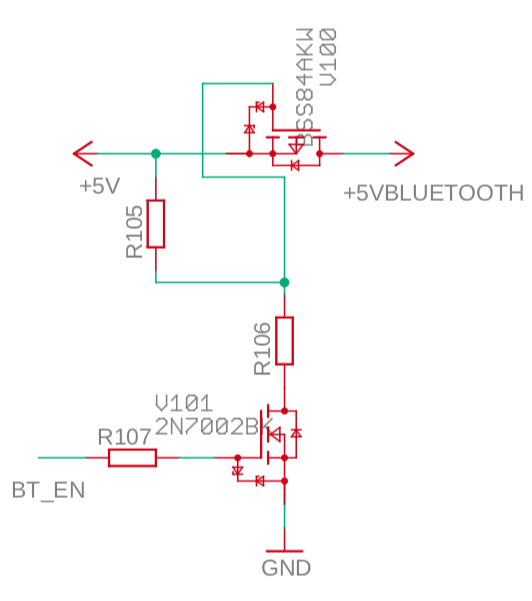
\includegraphics[width=0.4\textwidth]{./img/spannungsabschaltung.png}
  \caption{Spannngsabschaltung Bluetooth-Modul}\label{fig.spgsabschaltung}
\end{figure}

Bei einem Einschaltsignal über BT\_EN vom Mikrocontroller schaltet der n-Kanal-Mosfet V101 durch; der Spannungsteiler aus $R_{105}$ und $R_{106}$ ist aktiv. 
%5vgps, 5vbt, Mosfets, Spannungsteiler

\subsection{Messung Strom/Spannung}\label{subsec.MessungStromSpannung}
%Sensoren ACS, Spannungsteiler Ladespannungsmessung

\subsection{Beschaltung Sensoren}\label{subsec.BeschaltungSensoren}
%Olis Dokument zusammenfassen



